\section{V6}
\subsection{Exceptions and Interrupts}\label{Exceptions}
\begin{minipage}{10cm}
	Exceptions sind Ereignisse, die den sequenziellen Programmablauf ver"andern. Der Prozessor unterbricht den normal laufenden Programmablauf (Background) und f"uhrt einen Exception-Handler (Foreground) aus. Exceptions werden vom NVIC (nested vectored interrupt controller) verarbeitet. Der NVIC kann eine Reihe von  \textit{Interrupt Request (IRQs)} und einen \textit{Non-Maskable Interrupt (NMI)} verarbeiten, wobei der \textit{NMI} beispielsweise von einem Watchdog-Timer aktiviert werden kann. 
\end{minipage}
%
\begin{minipage}{0.5cm}
	\-\
\end{minipage}
%
\begin{minipage}{9cm}
	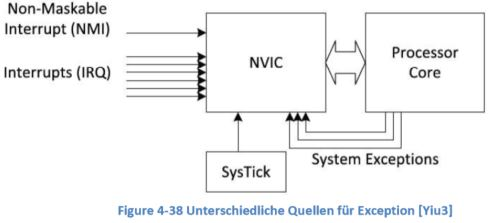
\includegraphics[width=8.5cm]{images/NVICExcp}
\end{minipage}

Der Prozessor selbest ist auch eine Quelle von Exceptions.\\
Jede Exception-Quelle hat eine zugeh"orige Exception-Number:
        \begin{itemize}
        	\item Exception-Number 1-15 gelten als \textit{System-Exceptions}
        	\item Exception-Number 16-255 sind \textit{Interrupts}
        \end{itemize} 
        Der NVIC kann bis zu 240 IRQs verarbeiten, in der Praxis sind es aber oft weniger.
    
Exception-Handler für Interrupts werden als Interrupt Service Routine (ISR) bezeichnet, wobei die Interrupt-Latenzzeit (\textit{Interrupt Latency}) gerade mal 12 Clockzyklen betr"agt.

\subsubsection{NVIC}
Jeder Interrupt kann individuell aktiviert/deaktiviert werden, ausserdem kann sein \textit{Pending State} durch die Software gesetzt/gel"oscht werden. Den Exceptions k"onnen \textit{Priority-Level} zugeordnet werden und somit ausgel"oste ISRs mit tieferer Priorit"at durch einen Interrupt h"oherer Priorit"at unterbrochen werden.
\subsection{Reset und Reset-Sequenzen}
\subsubsection{Reset}
Es gibt 3 Arten von Reset:\\
\begin{tabular}{ll}
    \textbf{Power-on Reset}  & Resettet den gesamten $\mu$ C, auch alle Peripherien und Debug-Komponenten \\ 
    \textbf{System Reset}    & Resettet nur den Prozessor und die Peripherien, aber nicht die Debug-Komponenten \\ 
    \textbf{Processoer Reset} & Resettet nur den Prozessor\\
\end{tabular}

\subsubsection{Reset Sequenz}
\begin{minipage}{9cm}
	Nach einem Reset und bevor der Cortex-M Prozessor mit der eigentlichen Programmausf"uhrung startet, liest die CPU die ersten beiden 32-Bit Word aus dem Speicher. Am Anfang in der Vektor-Tabelle steht der \textbf{Initial} \textit{Main-Stack-Pointer (MSP)} gefolgt vom \textbf{Initial} \textit{Program Counter (PC)}. Das Setup des MSP ist notwendig, um von Beginn weg einen g"ultigen Stack zu haben.
\end{minipage}
%
\begin{minipage}{0.5cm}
	\-\
\end{minipage}
%
\begin{minipage}{9cm}
	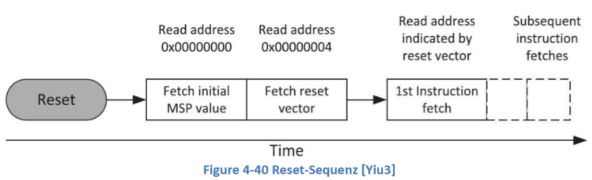
\includegraphics[width=9cm]{images/resetsequenz}
\end{minipage}

\subsection{Fault-Handling}
\begin{minipage}{9cm}
	Der Fault-Exception Mechanismus erlaubt eine schnelle Reaktion auf Systemfehler und gibt der Software die M"oglichkeit, Notfallszenarien einzuleiten. Standardm"assig sind die Exceptions \textit{Bus Fault, Usage Fault} und \textit{Memory Management Fault} deaktiviert, stattdessen triggern alle drei Faults die \textit{Hard Fault Exception}.
\end{minipage}
%
\begin{minipage}{0.5cm}
	\-\
\end{minipage}
%
\begin{minipage}{9cm}
	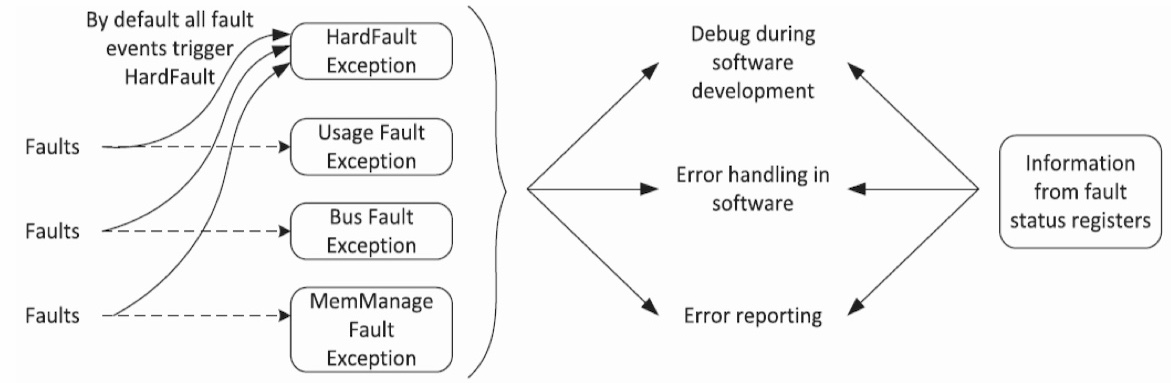
\includegraphics[width=9cm]{images/fault-handling}
\end{minipage}
    
\subsection{Spezial-Register}     
Register um Exceptions ein oder auszuschalten:\\
\textbf{$\rightarrow$ PRIMASK,FAULTMASK,BASEPRI}

\begin{minipage}{9cm}
    \subsubsection{PRIMASK}
    \begin{itemize}
        \item 1-bit Register
        \item Wenn das aktiv ist, werden NMI-Interrupts erlaubt
        \subitem $\rightarrow$ alle anderen Interrupts werden überdeckt
        \subitem $\rightarrow$ Default-Wert= 0, also deaktiviert
    \end{itemize}
 \end{minipage}
 %
 \begin{minipage}{0.5cm}
 	\-\
 \end{minipage}  
 %
 \begin{minipage}{9cm}
 	\subsubsection{FAULTMASK}
    \begin{itemize}
        \item 1-bit Register
        \item Wenn das aktiv ist, werden nur noch NMI-Interrups akzeptiert.\newline
        Alle anderen Interrupts und Exceptioln-Handlings werden deaktiviert
        \subitem $\rightarrow$ Default-Wert = 0
    \end{itemize}
 \end{minipage}

\subsubsection{BASEPRI}
\begin{itemize}
    \item Register das bis zu 8 Bits enthalten kann
    \item definiert eine Prioritätsstufe
    \item Hohe Stufe = Hohe Priorität
    \item Wenn das gesetzt wird, werden alle Interrupts mit gleicher oder tieferer Stufe deaktiviert
\end{itemize}

\subsubsection{Control-Register}
Das Kontroll-Register definiert:
\begin{enumerate}
    \item Die Auswahl zwischen MSP (Main-SP) und PSP (Process-SP)
    \item Die Zugriffsstufe und Thread-Mode
    \subitem (Ob Privilegd oder unprivilegd)
\end{enumerate}
\begin{multicols}{2}
    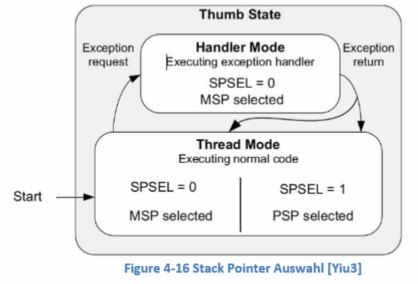
\includegraphics[width=\linewidth]{images/StackPointerAuswahl}
    
    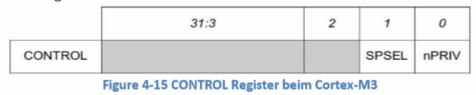
\includegraphics[width=\linewidth]{images/controlRegister}
\end{multicols}